\chapter{Introduktion}

Det kendte spil \textbf{Snake}, er et arkadespil, hvor spilleren bevæger en slange rundt på en bane og samler point for at forlænge slangen. Spillet er simpelt, men kan af denne grund have mange forskellige funktioner udover de sædvanlige, hvilket gør hver version ny og unik.
\newline

I denne rapport dokumenterer vi designet, implementeringen og evalueringen af vores egen version af Snake. Formålet med projektopgaven er at genskabe Snake som et Java-program, samt at dokumentere hvordan spillet er struktureret og udviklet, og hvorfor vi har valgt visse metoder og algoritmer.
Spillet er gengivet i to versioner: \textbf{Simple Snake} og \textbf{Advanced Snake}.
\newline

Simple Snake er en primitiv version af spillet, hvor styring og bevægelse kun foregår vha. input fra spilleren. Spillet opbygges efter \textit{Model-View-Controller}-designet, der gør det let at lave justeringer i spillet, når det senere skal udvides til Advanced Snake. Spillet er som navnet angiver simpelt og skal kun indeholde det mest essentielle for et snake-spil. Advanced Snake bygger videre på Simple Snake og bevarer derfor \textit{Model-View-Controller}-designet, men med tilføjede funktioner, der gør spillet mere udfordrende. Slangen skal kunne bevæge sig af sig selv, brugergrænsefladen skal udvides til at vise andet en blot spil-scenen og control-delen skal udvides til ikke blot at tage tastatur-input, men også musseklik-input. Klasserne er holdt så separate som muligt for at undgå for meget sammenblanding og indbyrdes afhængighed, hvor der ikke skal være det.
\newline

I rapporten vil designet samt implementeringen af begge spillets versioner blive forklaret. Først gennemgås den simple version, Simple Snake, hvor projektet først afgrænses til de funktioner og egenskaber, som vi har valgt at fokusere på. Derefter bestemmes i design-delen de metoder, som vi synes er bedst til at løse vores problemer, hvilket letter implementeringen. I implementerings-delen af rapporten, vil vi gå igennem implementeringen af Model- View- og Controller-delene hver for sig, og kort redegøre for deres sammenhæng. På samme måde gennemgås derefter Advanced Snake. I evaluerings-kapitlerne redegør vi for de tanker, valg og komplikationer som vi støder på undervejs. 

Vi brugt github til at strukturere vores samarbejde. Vores repositorie med commit historie og eventuel videre udbygning kan findes her
\begin{center}
\texttt{https://github.com/RandomInEqualities/Snake}
\end{center}

\begin{figure}
	\centering
	\subfloat[Simpel Snake]{\figlab{simplesnake}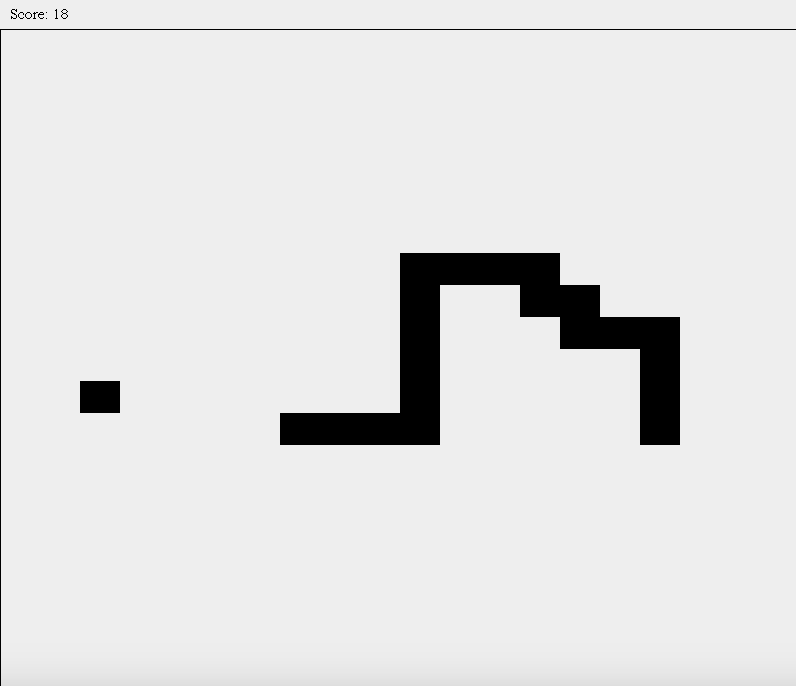
\includegraphics[width=0.30\textwidth]{SimpelSnake.png}}
	\hspace{0.1\textwidth}
	\subfloat[Avanceret Snake]{\figlab{advancedsnake}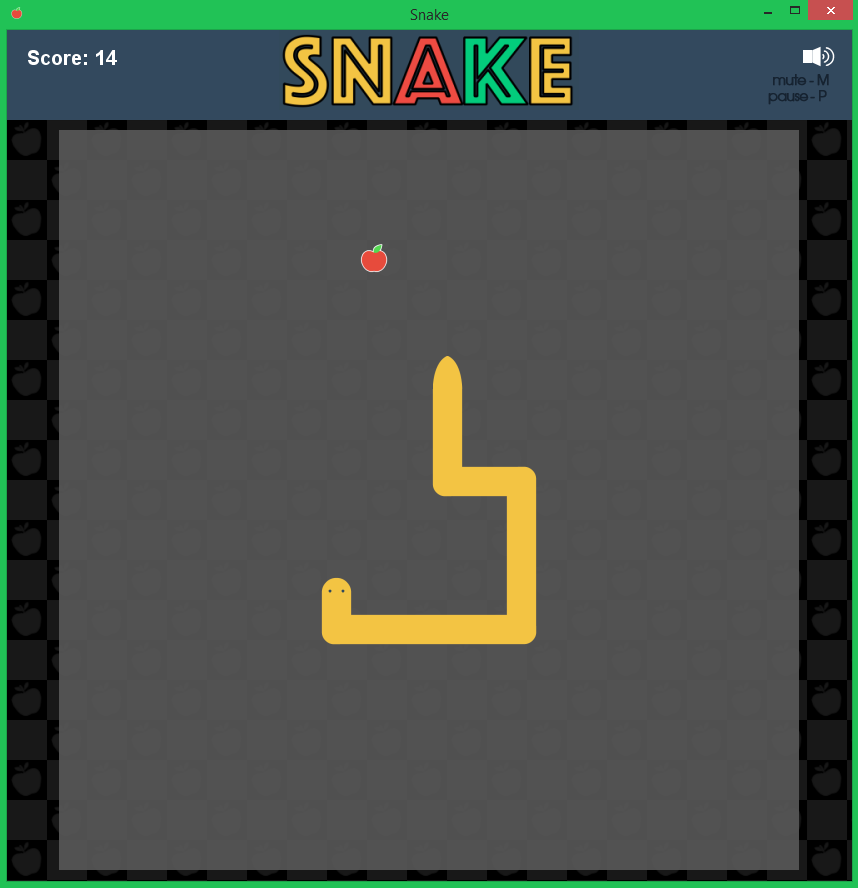
\includegraphics[width=0.33\textwidth]{AdvancedSnake.png}}
	\caption{\textit{Billede af Simple og Advanced Snake.}}
\end{figure}